\documentclass[12pt]{article}\usepackage[]{graphicx}\usepackage[]{color}
%% maxwidth is the original width if it is less than linewidth
%% otherwise use linewidth (to make sure the graphics do not exceed the margin)
\makeatletter
\def\maxwidth{ %
  \ifdim\Gin@nat@width>\linewidth
    \linewidth
  \else
    \Gin@nat@width
  \fi
}
\makeatother

\definecolor{fgcolor}{rgb}{0.345, 0.345, 0.345}
\newcommand{\hlnum}[1]{\textcolor[rgb]{0.686,0.059,0.569}{#1}}%
\newcommand{\hlstr}[1]{\textcolor[rgb]{0.192,0.494,0.8}{#1}}%
\newcommand{\hlcom}[1]{\textcolor[rgb]{0.678,0.584,0.686}{\textit{#1}}}%
\newcommand{\hlopt}[1]{\textcolor[rgb]{0,0,0}{#1}}%
\newcommand{\hlstd}[1]{\textcolor[rgb]{0.345,0.345,0.345}{#1}}%
\newcommand{\hlkwa}[1]{\textcolor[rgb]{0.161,0.373,0.58}{\textbf{#1}}}%
\newcommand{\hlkwb}[1]{\textcolor[rgb]{0.69,0.353,0.396}{#1}}%
\newcommand{\hlkwc}[1]{\textcolor[rgb]{0.333,0.667,0.333}{#1}}%
\newcommand{\hlkwd}[1]{\textcolor[rgb]{0.737,0.353,0.396}{\textbf{#1}}}%

\usepackage{framed}
\makeatletter
\newenvironment{kframe}{%
 \def\at@end@of@kframe{}%
 \ifinner\ifhmode%
  \def\at@end@of@kframe{\end{minipage}}%
  \begin{minipage}{\columnwidth}%
 \fi\fi%
 \def\FrameCommand##1{\hskip\@totalleftmargin \hskip-\fboxsep
 \colorbox{shadecolor}{##1}\hskip-\fboxsep
     % There is no \\@totalrightmargin, so:
     \hskip-\linewidth \hskip-\@totalleftmargin \hskip\columnwidth}%
 \MakeFramed {\advance\hsize-\width
   \@totalleftmargin\z@ \linewidth\hsize
   \@setminipage}}%
 {\par\unskip\endMakeFramed%
 \at@end@of@kframe}
\makeatother

\definecolor{shadecolor}{rgb}{.97, .97, .97}
\definecolor{messagecolor}{rgb}{0, 0, 0}
\definecolor{warningcolor}{rgb}{1, 0, 1}
\definecolor{errorcolor}{rgb}{1, 0, 0}
\newenvironment{knitrout}{}{} % an empty environment to be redefined in TeX

\usepackage{alltt}

\usepackage[utf8]{inputenc}
\usepackage[T1]{fontenc}
\usepackage[french]{babel}
\usepackage[hidelinks]{hyperref}
\usepackage{amsmath}
%\usepackage{fullpage}
%\usepackage{microtype}
\usepackage[backend=biber]{biblatex}
\usepackage{float}
\usepackage{csquotes}

\title{\textbf{Étude de marché pour les nouvelles gammes PSA Peugeot-Citroën}}
\author{Marc \textsc{Autrand}, Timothée \textsc{Pallot},\\*Edouard
	\textsc{Nguon}, Rémi \textsc{Nicole}}
\date{11 décembre 2015}

\addbibresource{liography.bib}
\IfFileExists{upquote.sty}{\usepackage{upquote}}{}
\begin{document}

\maketitle

\break
~
\newpage
\break
\tableofcontents

\part{Pré-enquête}

\section{Introduction}

\paragraph{} Dans le cadre de l'unité MSH-3001, nous avons réalisé une étude du
marché automobile, afin de répondre aux questions soulevées par la politique récente
du groupe PSA Peugeot-Citroën ; celle de la réponse du public au nouveau modèle
phare de Citroën, la C4 Cactus, et celle du futur de la marque DS. Quels développements
pourront connaître ces deux marques, l'une en pleine redéfinition, l'autre à l'assaut
d'une concurrence solidement ancrée dans les habitudes du public ?

\paragraph{} Notre enquête nous a tout d'abord amenés à discuter avec des professionnels,
et notamment des conseillers commerciaux de marques concurrentes. Nous avons ensuite
réalisé un sondage de plus grande ampleur auprès des clients potentiels des deux marques.

\paragraph{} Ce dernier a rassemblé plus de cent cinquante réponses, au sein de publics
différents tels que le monde étudiant ou les communautés d'automobilistes. Il nous a
permis de recueillir de nombreux commentaires sur le modèle Cactus, sur les plans fonctionnel
et esthétique. Nous avons également obtenu l'opinion du public sur la marque DS, désormais
indépendante, afin de connaître le positionnement qu'il lui donne sur le
marché haut de gamme.

\break
\section{Historique}

\paragraph{} L'histoire récente de PSA Peugeot-Citroën est marquée par
plusieurs bouleversements. Depuis le rachat de Citroën par Michelin en 1976, le
groupe doit relever le défi de faire cohabiter deux marques concurrentes. Si la
distinction claire entre les clients Citroën et Peugeot, creusée depuis les
années 1950, semblait être un avantage, le groupe parvient difficilement à
concilier les différences de culture et d'approche des deux constructeurs. Peu
à peu, il s'éloigne du marché haut de gamme, duquel Citroën était pourtant
proche.

\paragraph{} En 2009, le lancement de la gamme DS ouvre de nouveaux horizons.
Créé par le PDG sortant Christian Streiff, le label mise sur le retour très
populaire des anciens modèles phares des marques européennes : Mini Cooper,
Fiat 500, etc. Si le sigle DS apporte l'héritage de la gamme mythique des
années 1960, le design est celui d'une marque premium, tout comme le prix des
modèles. Citroën part ainsi à l'assaut de ténors comme Audi, mais aussi du
marché chinois, longtemps délaissé, pour lequel le prix a moins d'importance
que la qualité du véhicule.

\paragraph{} La ligne DS est un succès. Pour autant, sa communication l'éloigne
peu à peu de Citroën ; en 2014, le groupe PSA choisit d'en faire une filiale à part
entière. Ne reste alors plus à Citroën que sa seconde spécialité, celle de
faire du différent. Elle présente ainsi au même moment un modèle d'un genre
nouveau, entre la berline et le SUV, et doté d'un design particulier : la C4
Cactus, première d'une génération de voitures vouée à redéfinir la gamme
Citroën.

\paragraph{} Si la stratégie du groupe PSA depuis 2014 a été efficace, en
renouant dès le premier semestre 2015 avec les bénéfices\cite{lesechos}, le
futur est plus incertain. La C4 Cactus est un modèle clivant qui rassemble de
nombreux fans mais souffre d'un manque de reconnaissance du grand public. La
gamme DS, quant à elle, prend son envol en Chine et veut devenir le porte-étendard
du groupe.\\

\noindent \emph{Quel développement peuvent connaître ces deux gammes, et
	peuvent-elles coexister?}

\break
\section{Méthodologie}

\paragraph{} Dans les premiers moments de notre étude, nous avons souhaité recueillir
l'avis de plusieurs concessionnaires. Nous avons ainsi pu nous entretenir avec des
conseillers commerciaux issus de magasins Peugeot et Renault ; ceux-ci représentent
respectivement une concurrence indirecte et directe pour Citroën et DS. Ces échanges,
basés sur un premier questionnaire, étaient informels, afin de connaître l'avis personnel
de ces employés.

\paragraph{} Afin de recueillir le sentiment du public, nous avons enrichi notre
questionnaire en vue d'une publication sous forme de sondage en ligne. Il était
important d'y ajouter des éléments de contexte ainsi que des illustrations, afin que
les internautes moins renseignés sur les gammes Citroën et DS puissent également nous donner
leur opinion. Le sondage a été partagé sur les réseaux sociaux auprès des communautés Citroën,
puis auprès d'un large panel d'étudiants qui représentent le public futur des deux marques.

\paragraph{} Le positionnement de la Cactus, proche des SUV, lui donnant plus
de chances de trouver un public à l'étranger qu'en France, nous avons également
cherché des retours à l'international. Cette décision était confortée par les
prix reçus par le véhicule : voiture de l'année en Espagne et au Danemark, prix
du design du salon de l'automobile New York, etc. Nous avons ainsi rédigé une version du
sondage en langue anglaise, qui a reçu plus de trente réponses dans des communautés
internationales d'amateurs de voitures françaises. Si une majorité
de retours nous sont venus du Royaume-Uni, des réponses ont aussi été données
depuis le Brésil, la Turquie et plusieurs pays européens.\\

\noindent Le total de personnes interrogées s'élève à plus de 150.

\part{Résultats}

\section{Retour des échanges avec les concessionnaires}

\paragraph{} Nous avons pu interroger deux conseillers commerciaux de
concessions Peugeot et Renault, le premier étant partenaire de Citroën au
sein du groupe PSA, et le second un concurrent de la marque.

\paragraph{} Le conseiller de Renault, âgé d'une vingtaine d'années et ne se voyant
pas comme un client fidèle de Renault, a dressé un portrait négatif de la
C4 Cactus. Il n'est pas du tout satisfait du design de ce modèle, trouvant les
air-bumps disgracieux et peu efficaces.
Il nous a confié avoir travaillé dans la production automobile, et avoir vu
beaucoup de C4 Cactus revenir au garage à cause des air-bumps, qui lorsqu'ils
sont endommagés nécessitent de changer les deux portes que le coussin relie
ainsi que le plastique autour d'elles, ce qui demande beaucoup de temps et de main d'œuvre.
D'après lui, la partie avant du véhicule ressemble à celle d'un $4 \times 4$,
ce qui la rend trop imposante et ne correspond pas aux habitudes de la marque Citroën.

\paragraph{} En ce qui concerne la marque DS, son avis est totalement
différent. Pour lui, le design des voitures de la marque est très réussi,
et il apprécie la décision de la nouvelle marque de se séparer de
Citroën. Cependant, les prix affichés par DS lui semblent trop élevés pour prétendre
atteindre des ventes aussi importantes que celles de ses concurrents.

\paragraph{} L'employé de Peugeot a également une mauvaise opinion du modèle Cactus.
Selon lui, le design de cette voiture est en décalage avec le style Citroën. La
technologie air-bump ne lui paraît pas révolutionnaire, et il se dit étonné
de la promotion faite par Citroën de ce procédé.

\paragraph{} Quant à la ligne DS, le conseiller reconnaît qu'elle a produit de très bons
produits tels que la DS3 et la DS4, mais la DS4 lui paraît trop proche de la Citroën
C4 : en dehors des phares, les deux voitures seraient identiques.
Pour lui, la marque DS souffre de plusieurs problèmes : le premier est que les
premières DS et notamment les plus médiatisées DS3 et DS4 ont été vendues par
Citroën, et non par DS. Le deuxième est sa politique de prix : elle fournit des
voitures à prix élevés de l'ordre de ceux des véhicules produits par Audi ou BMW,
mais pas de la même qualité.

\paragraph{} De plus, le conseiller accuse Citroën d'avoir voulu aller trop vite ; la marque ne serait
reconnue ni comme un constructeur de voiture de luxe, ni comme une marque adaptée
à un public jeune. Elle se voudrait en avance sur son temps, mais se serait essoufflée.
Le conseiller prend pour exemple la Peugeot 3008, qui aurait été conçue quatre ans
avant sa commercialisation ; Peugeot aurait ainsi anticipé les besoins futurs du public
et attendu sa maturité pour proposer son modèle.

\paragraph{} Enfin, le dernier problème de DS se situerait dans ses garages :
ceux-ci ne seraient pas reconnus pour leur qualité, malgré le positionnement
luxe donné par PSA à la marque DS.

\section{État des ventes de la Cactus et de DS, publics concernés}

\subsection{Citroën C4 Cactus}

\paragraph{} Après sa mise en vente en 2014, la C4 Cactus connaît un début
discret mais réussit tout de même à enregistrer 75 000
ventes au bout d'un an ainsi que 35 distinctions à travers le
monde\cite{communique}. Parmi ces véhicules, seuls 27\% ont été vendus en France.
Les Français sont beaucoup moins attirés par ce modèle, qui n'a pas été
commandé plus de 20 000 fois depuis son lancement en juin 2014 et a été vendu
à seulement 6 000 exemplaires en cette année 2015. Il faut également confronter à
ces chiffres les modèles confiés par Citroën à ses agents, et les stocks des
concessionnaires. La C4 Cactus parvient finalement à la 22\ieme{} place des voitures
les plus vendues en France depuis le début de l'année 2015.

\paragraph{} Ce modèle allie confort et technologie utile, et vise un public
préférant une voiture utile à un produit permettant d'affirmer son statut
social. En termes de prix, la Citroën Cactus se positionne entre les lignes ``low
cost'' et haut de gamme. En effet, son prix peut varier entre 15 200 €
et 22 900 € à neuf selon la finition et le moteur choisi\cite{banquette}.

\subsection{Ligne DS}

\paragraph{} La marque DS a connu son véritable lancement avec la DS3 en 2010 qui a
été vendue en 26 417 exemplaires cette même année, 33 015 l'année suivante,
puis les ventes ont diminué avec 25 107 ventes en 2012 et enfin 19 672 et 17 471
respectivement en 2013 et 2014. Ce modèle a plu à de nombreux clients de par
son design novateur\cite{avis}, son comportement routier exceptionnel, son
confort mais aussi son intérieur original et moderne. Les finitions sont
satisfaisantes, la voiture est très personnalisable, a une bonne habitabilité à
l'arrière et n'est pas très chère par rapport à ce que propose déjà Citroën,
puisque ces modèles s'articulent autour de 20 000 € pour les plus chers d'entre eux.

\paragraph{} En revanche, les clients lui reprochent quelques défauts comme un équipement
peu développé, la partie plastique qui n'est pas d'une grande qualité, et
des bruits parasites venant de temps en temps agacer le conducteur. Le
dernier point noir de ce modèle se situe au niveau des vitres arrières qui ne
peuvent pas s'ouvrir. La DS4 vient s'ajouter au marché en 2011, soit un an après
la sortie de son aînée et elle ne suscite pas autant d'admiration chez les
clients, car les ventes n'arrivent pas à décoller : 10 757 voitures vendues lors
de la première année, pour atteindre le pic de ventes l'année d'après avec 14
143 modèles vendus et retomber à 11 740 et 8 661 ventes en 2013 et 2014.

\paragraph{} La DS5 fait même moins de ventes que la DS4 puisque le nombre
maximum de voitures vendues sur une année est de 10 943, et concerne l'année de
sa sortie. Les deux années suivantes sont très mauvaises, les ventes tombant
à 8 365 en 2013 et 5 614 en 2014. En effet les défauts de la DS3 ne sont pas résolus,
à l'exception de l'équipement de la voiture. Le confort global est lui beaucoup
moins apprécié sur les DS4 et DS5 que sur la DS3.

\paragraph{} Cette nouvelle marque se distingue beaucoup de Citroën dans son
design, son luxe mais aussi son prix. Elle ne touche plus le très grand public,
mais se rapproche plus des marques allemandes telles que Audi et BMW. Elle
plaît également aux jeunes, qui sont attirés par son style, son design, ses
couleurs.

\break
\part{Analyse des résultats du sondage}

\section{Âge et sexe}



\begin{knitrout}
\definecolor{shadecolor}{rgb}{0.969, 0.969, 0.969}\color{fgcolor}\begin{figure}[H]
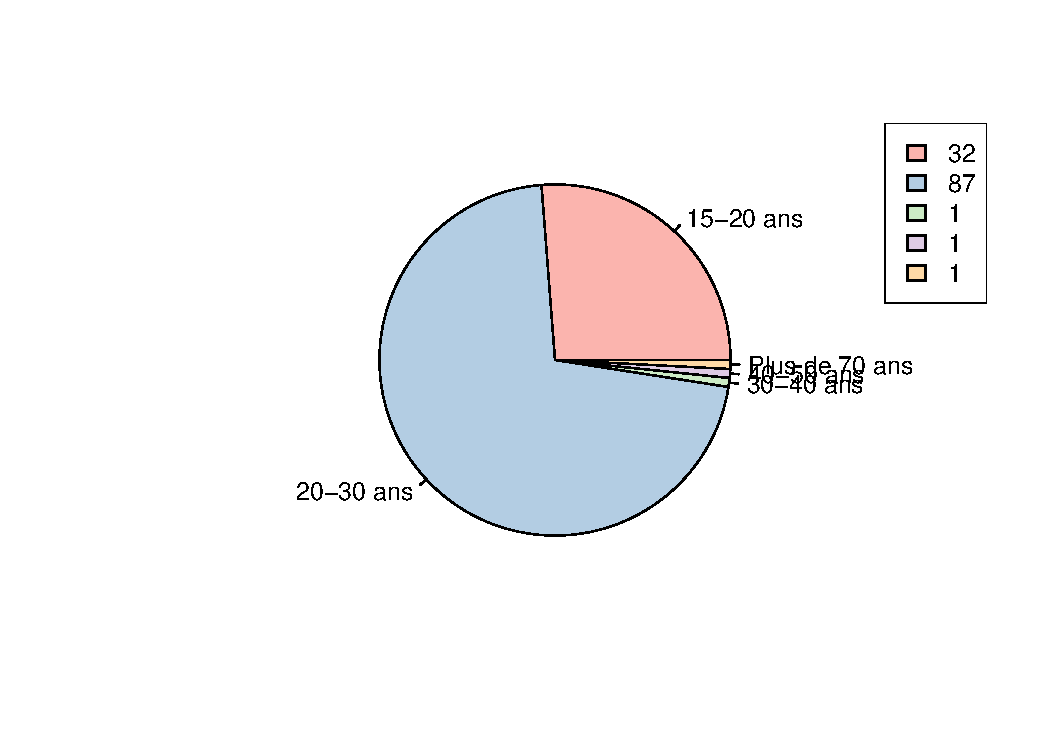
\includegraphics[width=\maxwidth]{figure/tranche_age_fr-1} \caption[Tranches d'âges des personnes ayant répondu au sondage français]{Tranches d'âges des personnes ayant répondu au sondage français}\label{fig:tranche age fr}
\end{figure}


\end{knitrout}
\paragraph{} Notre sondage en français ayant été partagé sur les
réseaux sociaux, et notamment au sein de groupes étudiants, la plupart de nos
réponses vient d'un public jeune (15-30 ans).

\begin{knitrout}
\definecolor{shadecolor}{rgb}{0.969, 0.969, 0.969}\color{fgcolor}\begin{figure}[H]
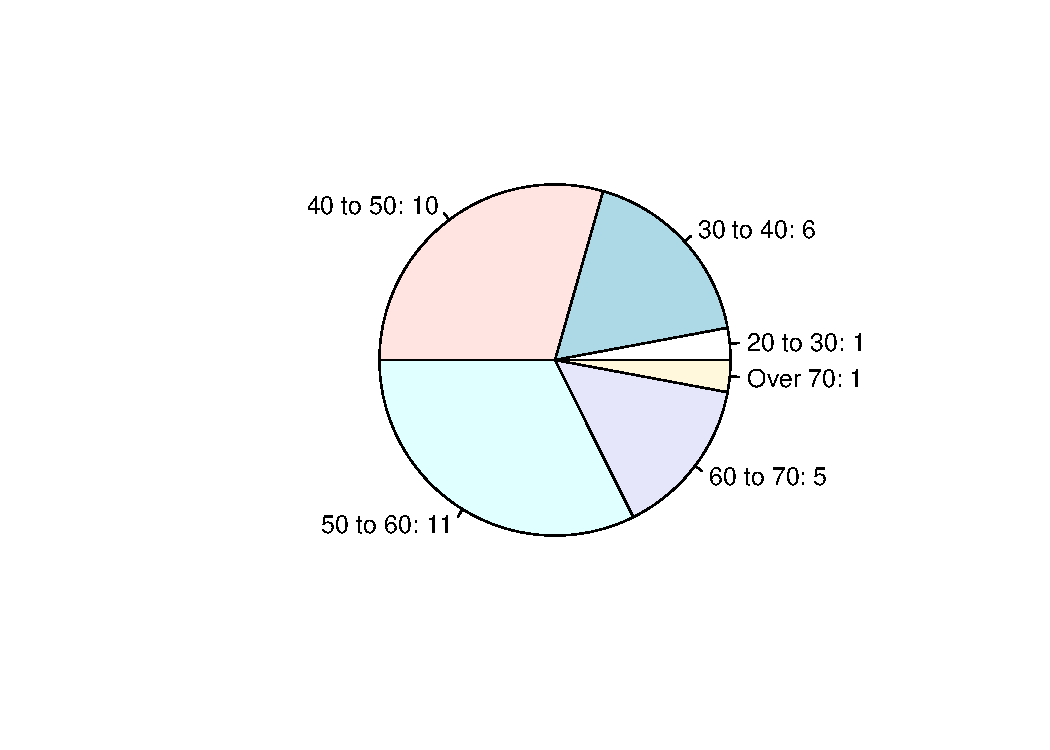
\includegraphics[width=\maxwidth]{figure/tranche_age_en-1} \caption[Tranches d'âges des personnes ayant répondu au sondage anglais]{Tranches d'âges des personnes ayant répondu au sondage anglais}\label{fig:tranche age en}
\end{figure}


\end{knitrout}

\paragraph{} Les tranches d'âges des personnes ayant répondu à notre sondage
en langue anglaise sont beaucoup plus réparties, même si la tendance est aux
individus de plus de 40 ans. Ceux-ci représentent 79\% des personnes ayant
répondu à cette enquête.

%\begin{knitrout}
%\definecolor{shadecolor}{rgb}{0.969, 0.969, 0.969}\color{fgcolor}\begin{figure}[H]
%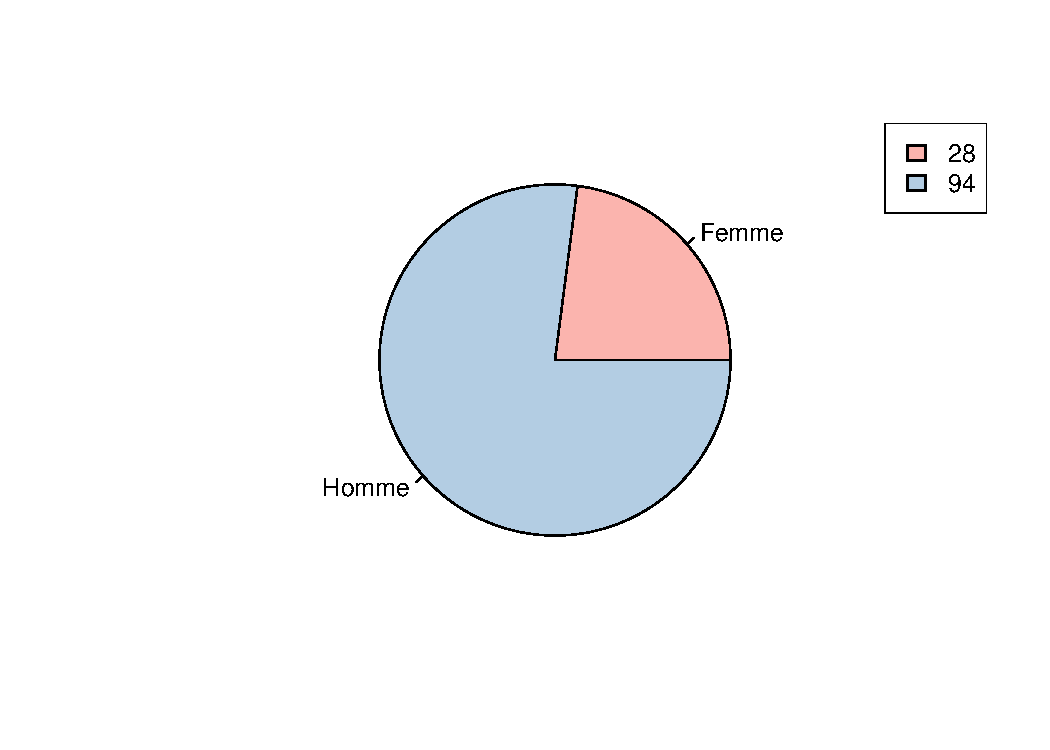
\includegraphics[width=\maxwidth]{figure/sexe_fr-1} \caption[Sexe des personnes ayant répondu au sondage français]{Sexe des personnes ayant répondu au sondage français}\label{fig:sexe fr}
%\end{figure}
%
%
%\end{knitrout}
%
%\begin{knitrout}
%\definecolor{shadecolor}{rgb}{0.969, 0.969, 0.969}\color{fgcolor}\begin{figure}[H]
%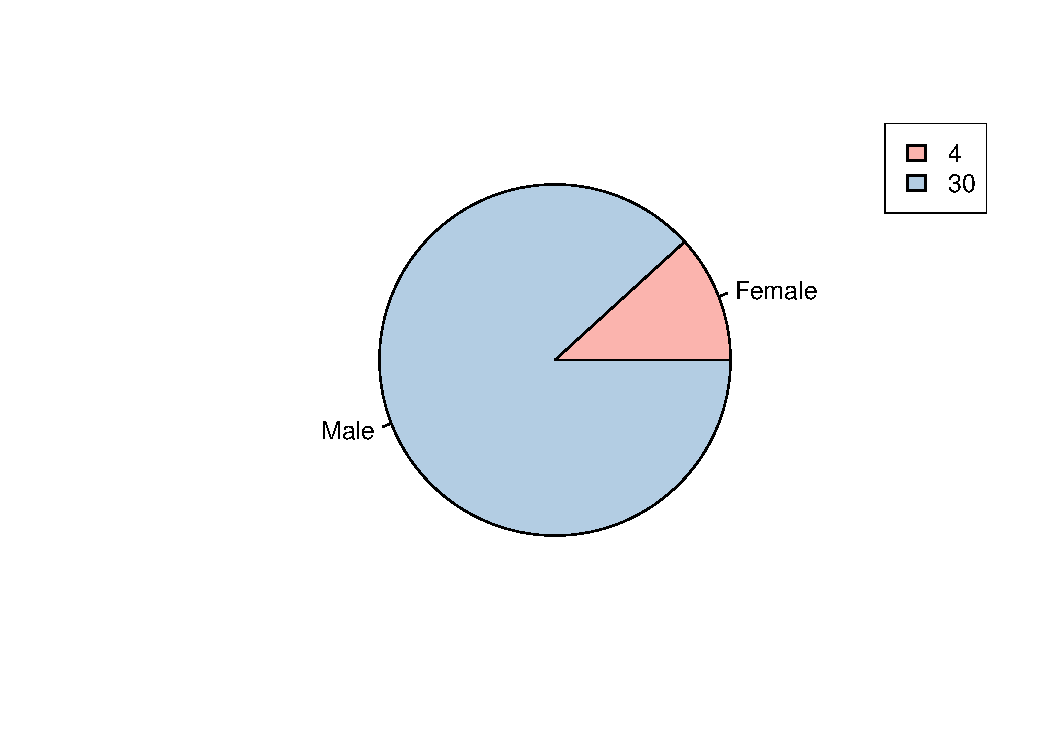
\includegraphics[width=\maxwidth]{figure/sexe_en-1} \caption[Sexe des personnes ayant répondu au sondage anglais]{Sexe des personnes ayant répondu au sondage anglais}\label{fig:sexe en}
%\end{figure}
%
%
%\end{knitrout}

\paragraph{} Parmi toutes les personnes ayant répondu à notre sondage, on peut noter
que seules 32 sur 156 sont des femmes, soit 21\%.

\break
\section{Marketing}

\begin{knitrout}
\definecolor{shadecolor}{rgb}{0.969, 0.969, 0.969}\color{fgcolor}\begin{figure}[H]
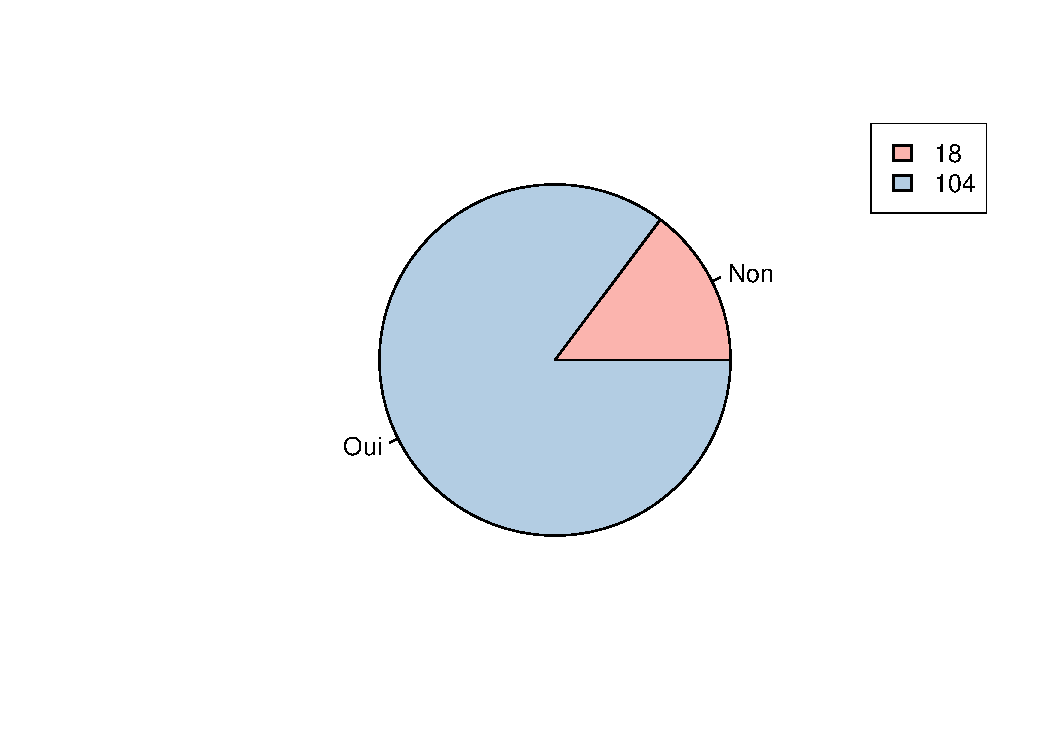
\includegraphics[width=\maxwidth]{figure/know_fr-1} \caption[Proportion des personnes connaissant auparavant la C4 Cactus ayant répondu au sondage français]{Proportion des personnes connaissant auparavant la C4 Cactus ayant répondu au sondage français}\label{fig:know fr}
\end{figure}


\end{knitrout}

%\begin{knitrout}
%\definecolor{shadecolor}{rgb}{0.969, 0.969, 0.969}\color{fgcolor}\begin{figure}[H]
%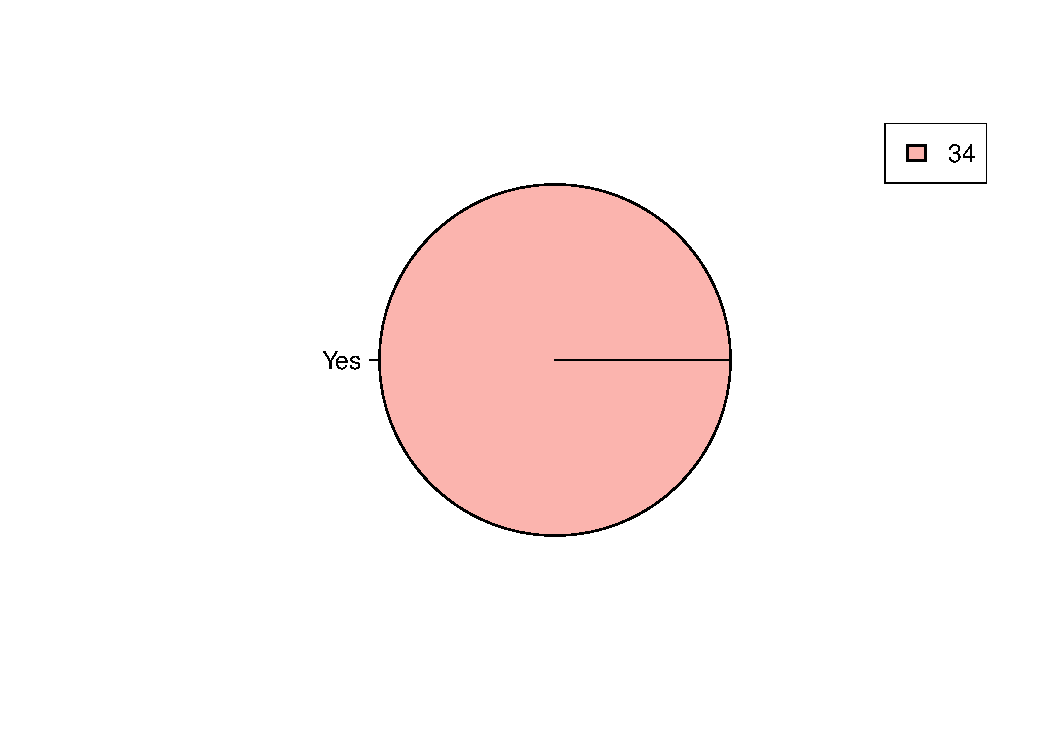
\includegraphics[width=\maxwidth]{figure/know_en-1} \caption[Proportion des personnes connaissant auparavant la C4 Cactus ayant répondu au sondage anglais]{Proportion des personnes connaissant auparavant la C4 Cactus ayant répondu au sondage anglais}\label{fig:know en}
%\end{figure}
%
%
%\end{knitrout}

\paragraph{} Si le sondage anglais, posté sur des communautés d'amateurs de voitures
françaises, montre que tous les sondés connaissaient auparavant le modèle Cactus,
le constat est différent en France où 15\% des personnes sondées ne le connaissent pas.


%\begin{knitrout}
%\definecolor{shadecolor}{rgb}{0.969, 0.969, 0.969}\color{fgcolor}\begin{figure}[H]
%
\includegraphics[width=\maxwidth]{figure/means_fr-1} \caption[Nuage de mots du moyen de prise de conscience de l'existence de la C4 Cactus des personnes ayant répondu au sondage français]{Nuage de mots du moyen de prise de conscience de l'existence de la C4 Cactus des personnes ayant répondu au sondage français}\label{fig:means fr}
%\end{figure}
%
%
%\end{knitrout}
%
%\begin{knitrout}
%\definecolor{shadecolor}{rgb}{0.969, 0.969, 0.969}\color{fgcolor}\begin{figure}[H]
%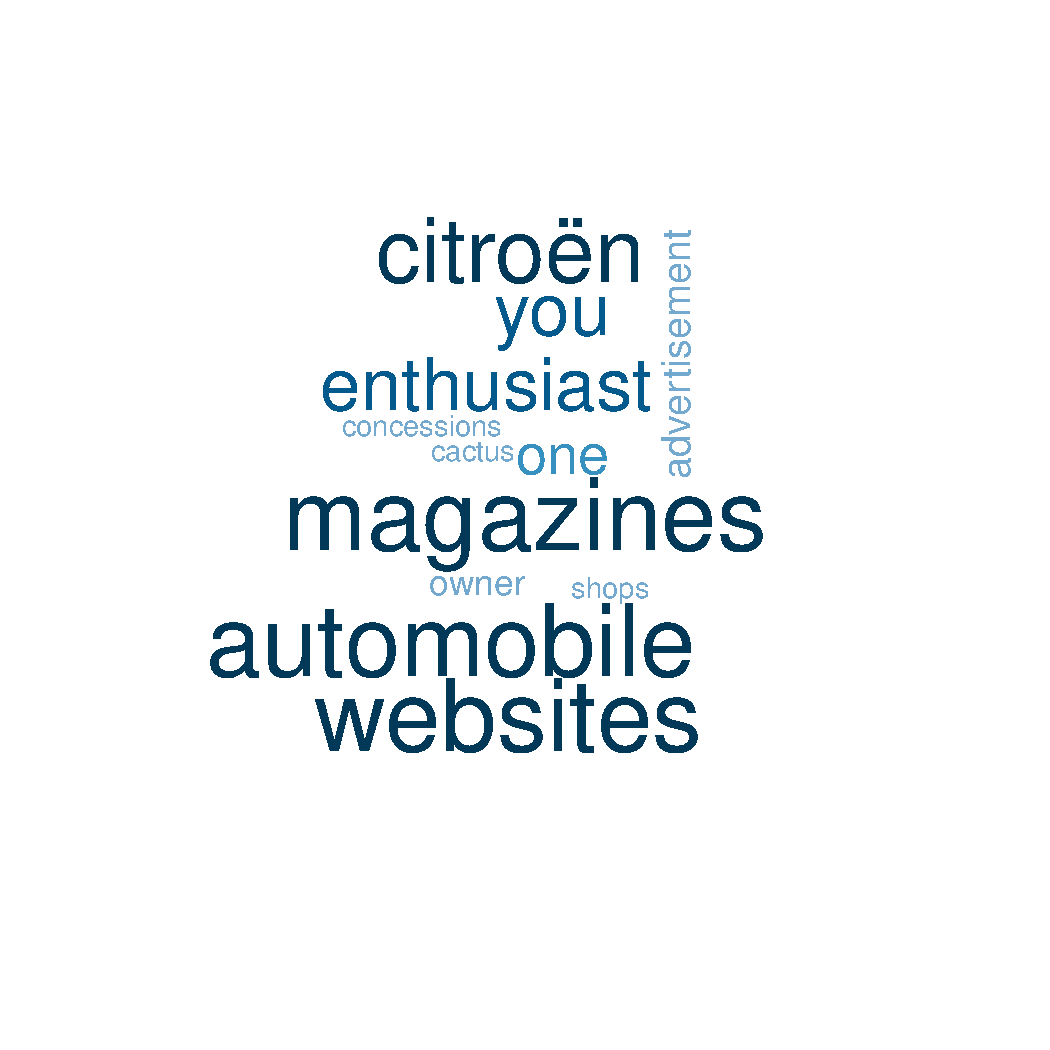
\includegraphics[width=\maxwidth]{figure/means_en-1} \caption[Nuage de mots du moyen de prise de conscience de l'existence de la C4 Cactus des personnes ayant répondu au sondage anglais]{Nuage de mots du moyen de prise de conscience de l'existence de la C4 Cactus des personnes ayant répondu au sondage anglais}\label{fig:means en}
%\end{figure}
%
%
%\end{knitrout}

\paragraph{} Les réponses à la question "Par quel moyen avez-vous entendu parler de la Cactus"
démontrent que la majorité des individus français connaissent la C4 Cactus grâce aux publicités,
aux magazines et à Internet. Les réponses en anglais sont issues d'un public toujours conscient des
derniers modèles des marques françaises.

\break
\section{Apparence de la voiture}

\begin{knitrout}
\definecolor{shadecolor}{rgb}{0.969, 0.969, 0.969}\color{fgcolor}\begin{figure}[H]
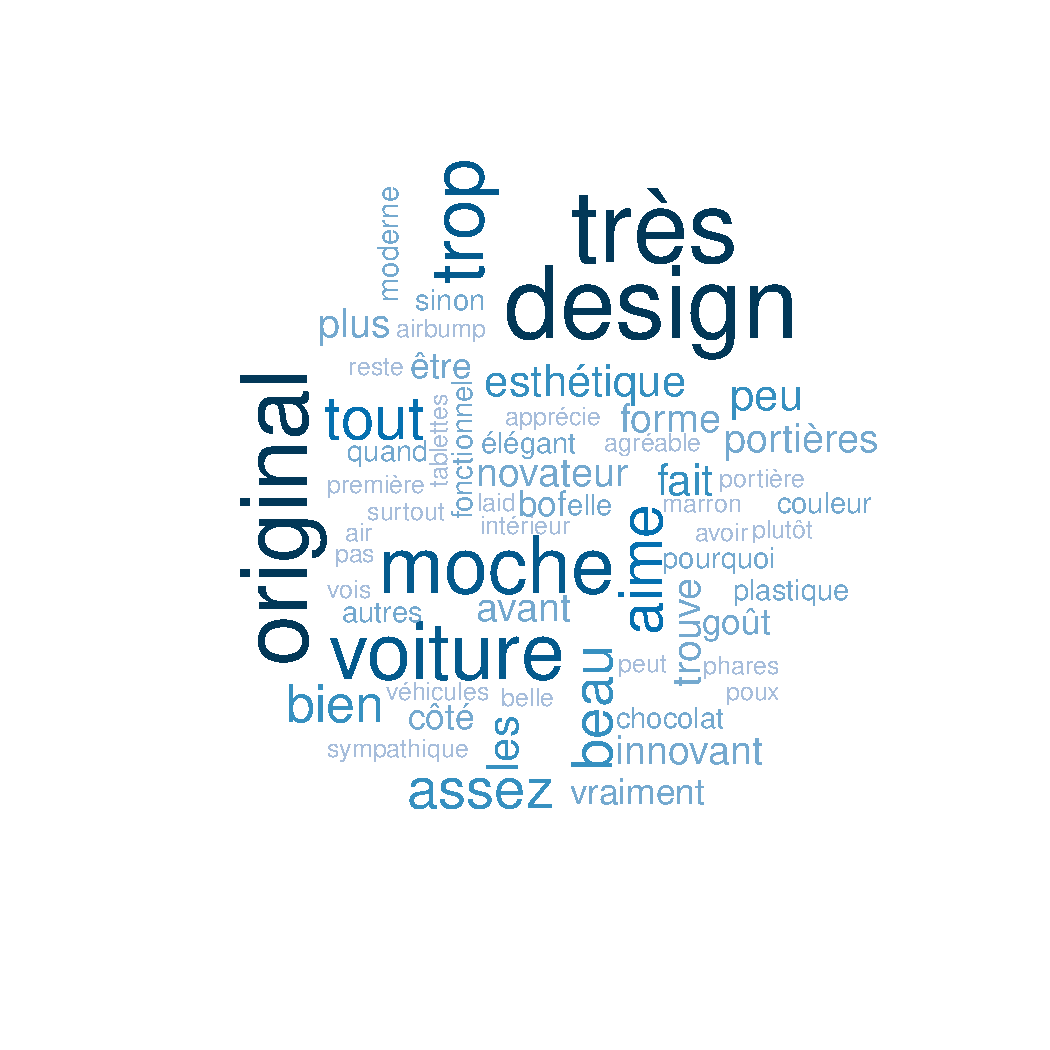
\includegraphics[width=\maxwidth]{figure/design_fr-1} \caption[Nuage de mots de l'avis sur le design de la C4 Cactus des personnes ayant répondu au sondage français]{Nuage de mots de l'avis sur le design de la C4 Cactus des personnes ayant répondu au sondage français}\label{fig:design fr}
\end{figure}


\end{knitrout}

\begin{knitrout}
\definecolor{shadecolor}{rgb}{0.969, 0.969, 0.969}\color{fgcolor}\begin{figure}[H]
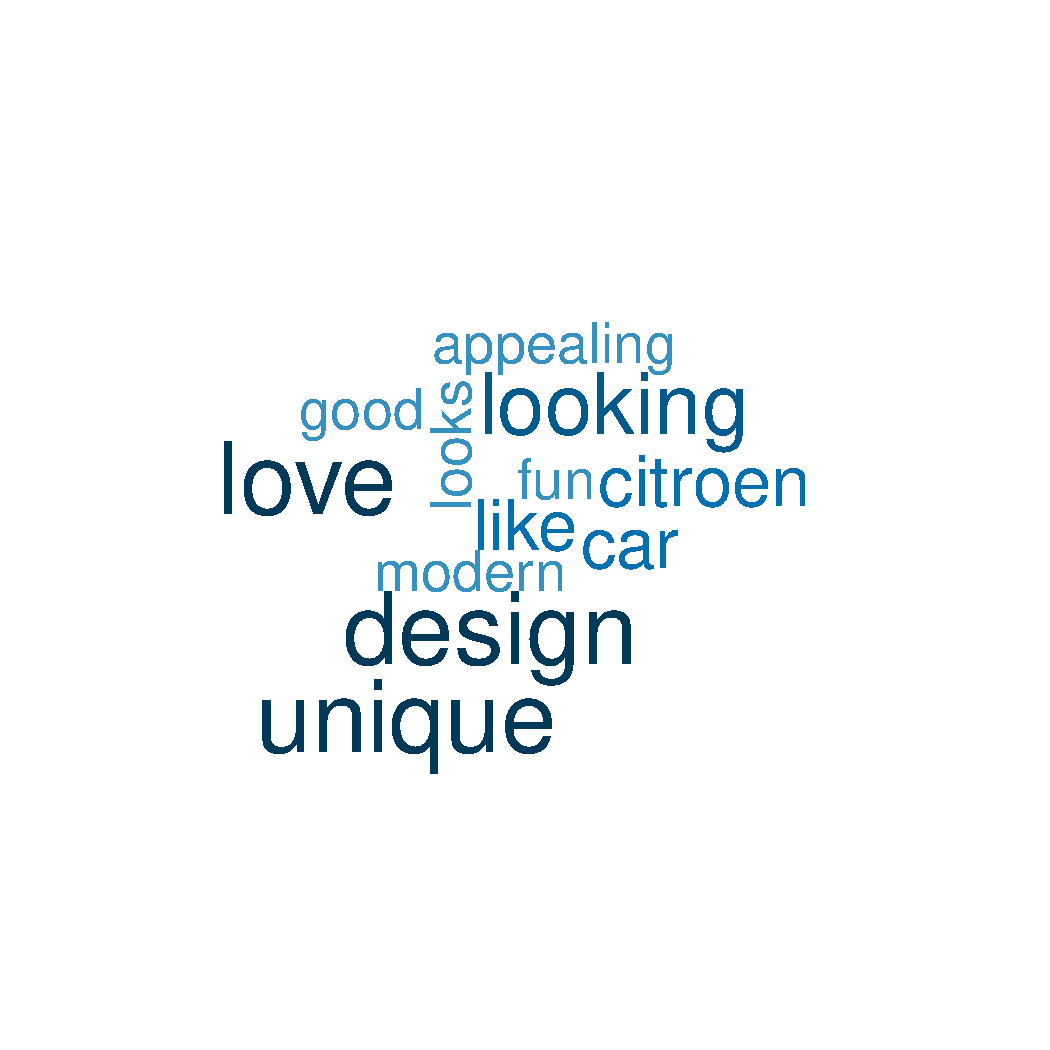
\includegraphics[width=\maxwidth]{figure/design_en-1} \caption[Nuage de mots de l'avis sur le design de la C4 Cactus des personnes ayant répondu au sondage anglais]{Nuage de mots de l'avis sur le design de la C4 Cactus des personnes ayant répondu au sondage anglais}\label{fig:design en}
\end{figure}


\end{knitrout}

\paragraph{} Les avis sur le design de la C4 Cactus sont assez partagés chez
les Français : on retrouve le plus souvent les termes ``très original'',
``design'', ``esthétique'', ``beau'', mais aussi ``moche''. Les Britanniques sont
quant à eux très flatteurs vis-à-vis du modèle.

\begin{knitrout}
\definecolor{shadecolor}{rgb}{0.969, 0.969, 0.969}\color{fgcolor}\begin{figure}[H]
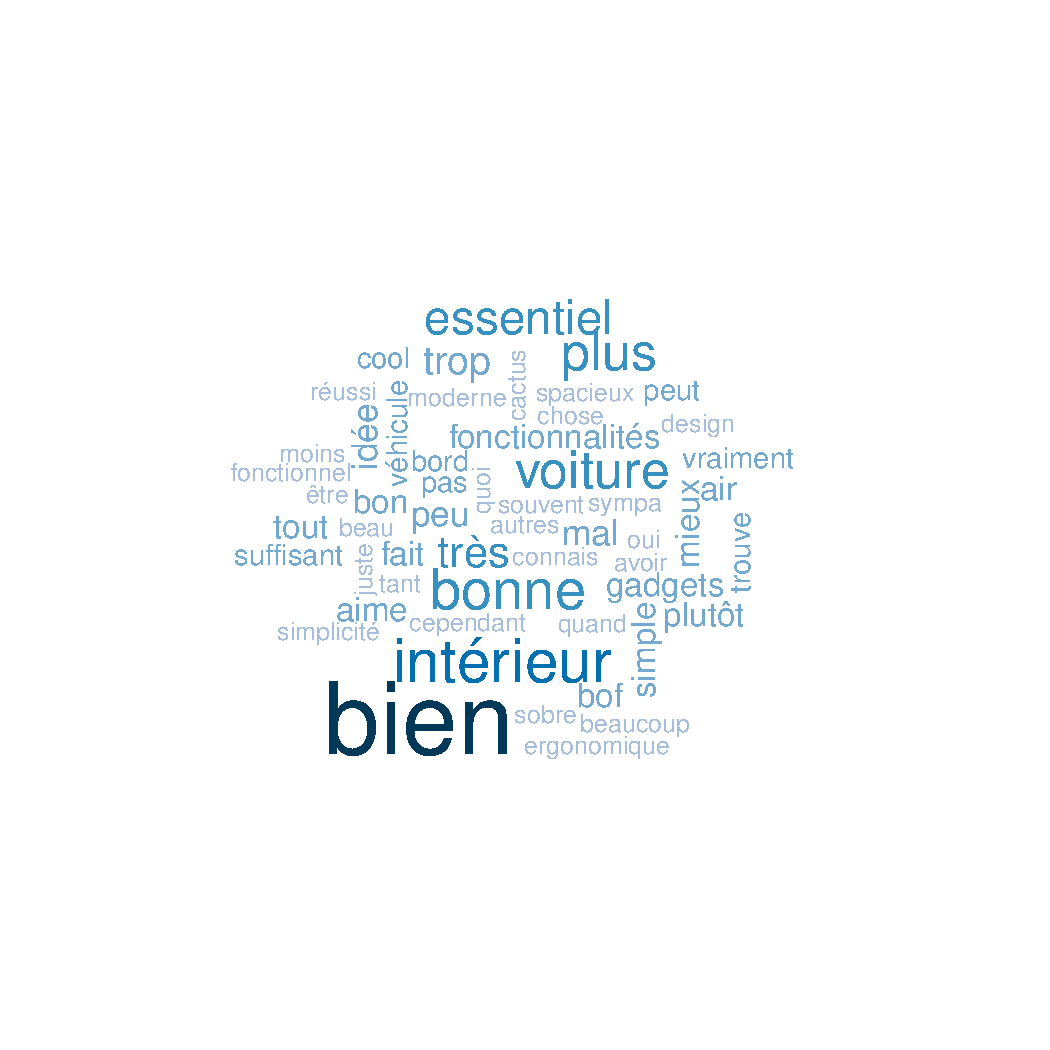
\includegraphics[width=\maxwidth]{figure/interior_fr-1} \caption[Nuage de mots de l'avis sur l'intérieur de la C4 Cactus des personnes ayant répondu au sondage français]{Nuage de mots de l'avis sur l'intérieur de la C4 Cactus des personnes ayant répondu au sondage français}\label{fig:interior fr}
\end{figure}


\end{knitrout}

%\begin{knitrout}
%\definecolor{shadecolor}{rgb}{0.969, 0.969, 0.969}\color{fgcolor}\begin{figure}[H]
%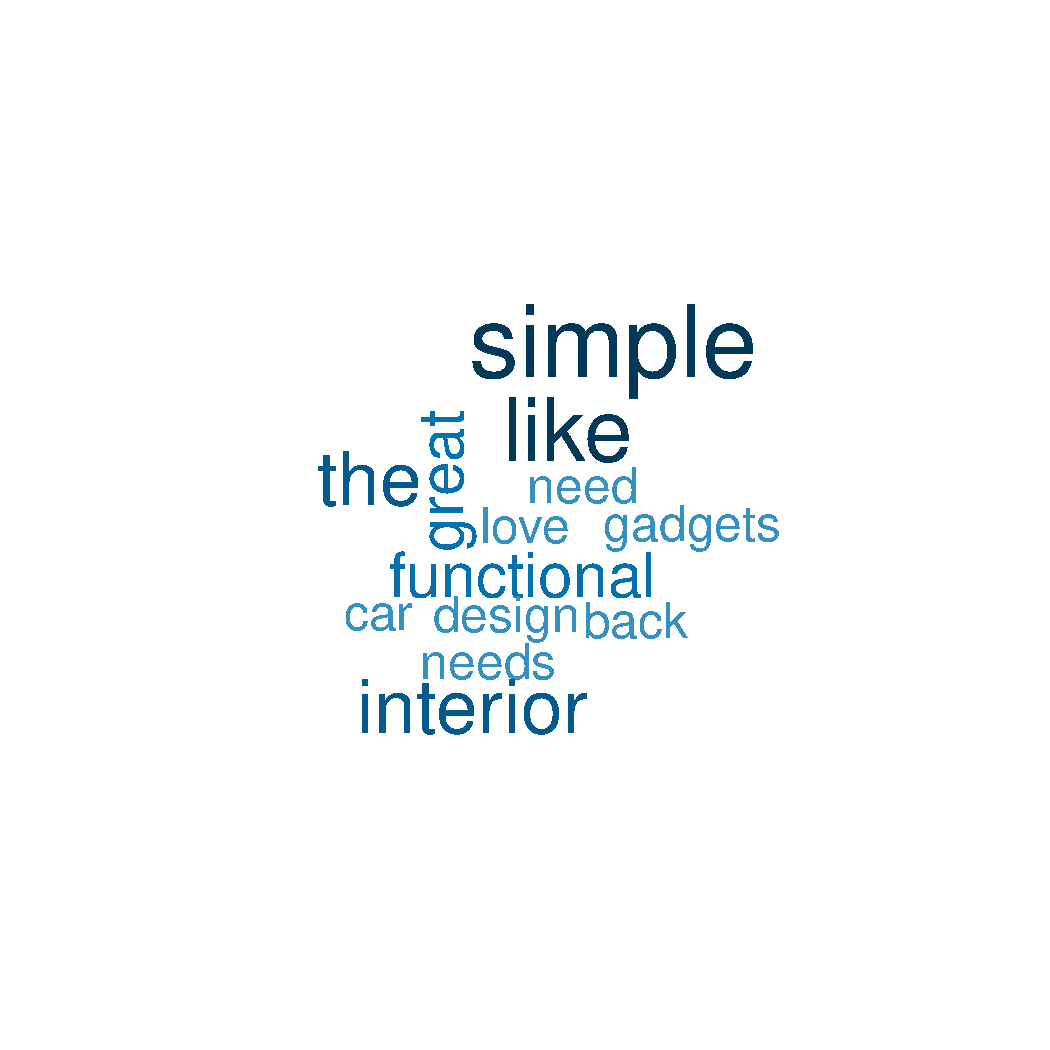
\includegraphics[width=\maxwidth]{figure/interior_en-1} \caption[Nuage de mots de l'avis de l'intérieur de la C4 Cactus des personnes ayant répondu au sondage anglais]{Nuage de mots de l'avis de l'intérieur de la C4 Cactus des personnes ayant répondu au sondage anglais}\label{fig:interior en}
%\end{figure}
%
%
%\end{knitrout}

\paragraph{} Concernant l'intérieur de la voiture, les termes ``bien'',
``bonne'', mais aussi ``simple'', ``great'', ``like'' reviennent très souvent, ce
qui montre que l'intérieur du modèle est très apprécié par les clients, non
seulement les loyaux anglais, mais aussi plusieurs français dont l'attrait pour
la voiture n'est pourtant pas unanime.

\break
\section{Opinion générale}



\begin{knitrout}
\definecolor{shadecolor}{rgb}{0.969, 0.969, 0.969}\color{fgcolor}\begin{figure}[H]
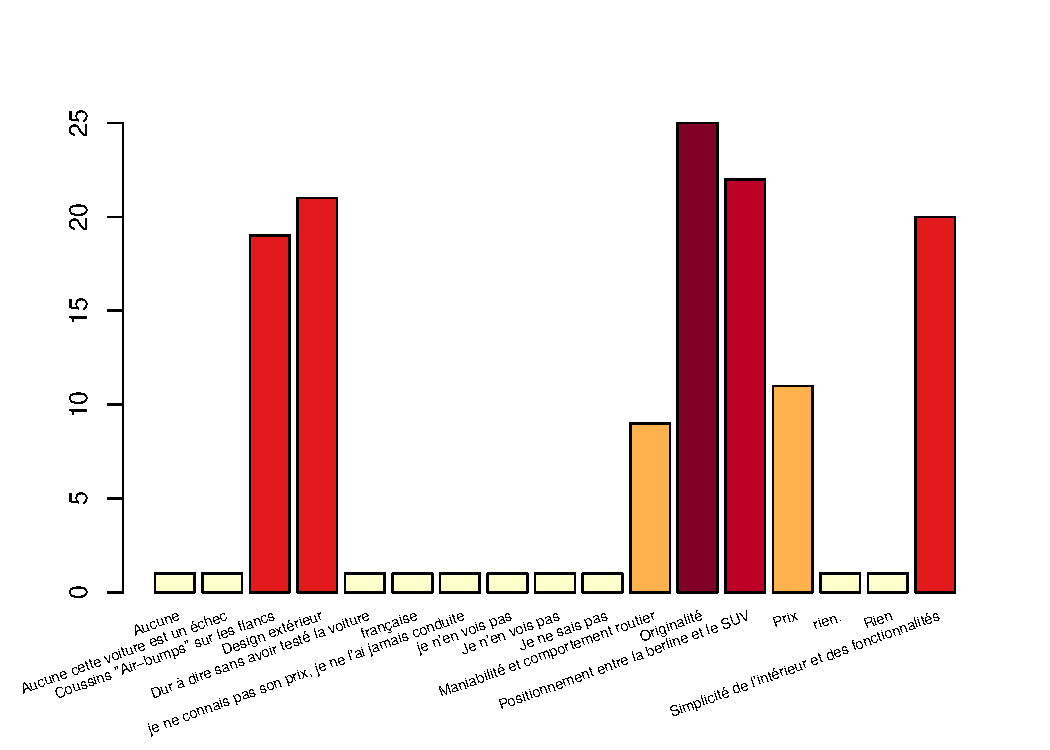
\includegraphics[width=\maxwidth]{figure/qualities_fr-1} \caption[Qualités de la C4 Cactus selon les personnes ayant répondu au sondage français]{Qualités de la C4 Cactus selon les personnes ayant répondu au sondage français}\label{fig:qualities fr}
\end{figure}


\end{knitrout}

\begin{knitrout}
\definecolor{shadecolor}{rgb}{0.969, 0.969, 0.969}\color{fgcolor}\begin{figure}[H]
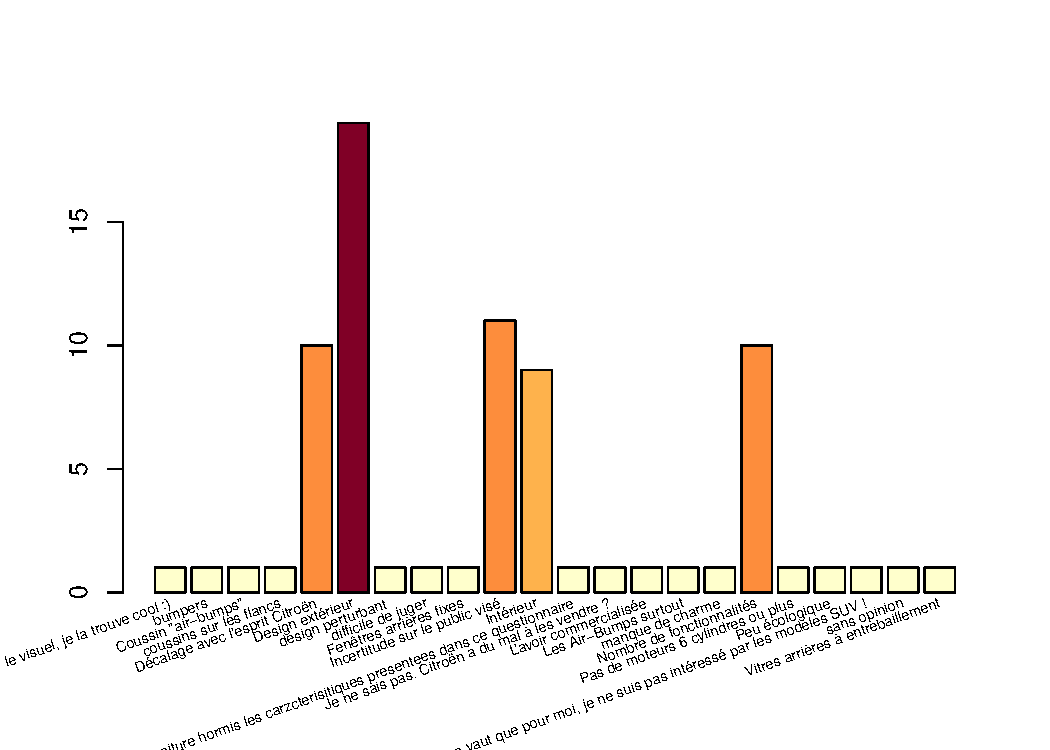
\includegraphics[width=\maxwidth]{figure/flaws_fr-1} \caption[Défauts de la C4 Cactus selon les personnes ayant répondu au sondage français]{Défauts de la C4 Cactus selon les personnes ayant répondu au sondage français}\label{fig:flaws fr}
\end{figure}


\end{knitrout}

\paragraph{} Les Français sont aussi très partagés dans les qualités et défauts
de la C4 Cactus. Plus de 20 personnes ont répondu que son originalité, son
design extérieur, la simplicité de son intérieur et de ses fonctionnalités, et
ses coussins ``airbump'' constituent ses qualités, alors que 24 personnes
pensent que son design extérieur est son
principal défaut. L'incertitude sur le public visé et le décalage avec l'esprit
Citroën sont les deux autres principaux défauts remarqués par les
Français.

\begin{knitrout}
\definecolor{shadecolor}{rgb}{0.969, 0.969, 0.969}\color{fgcolor}\begin{figure}[H]
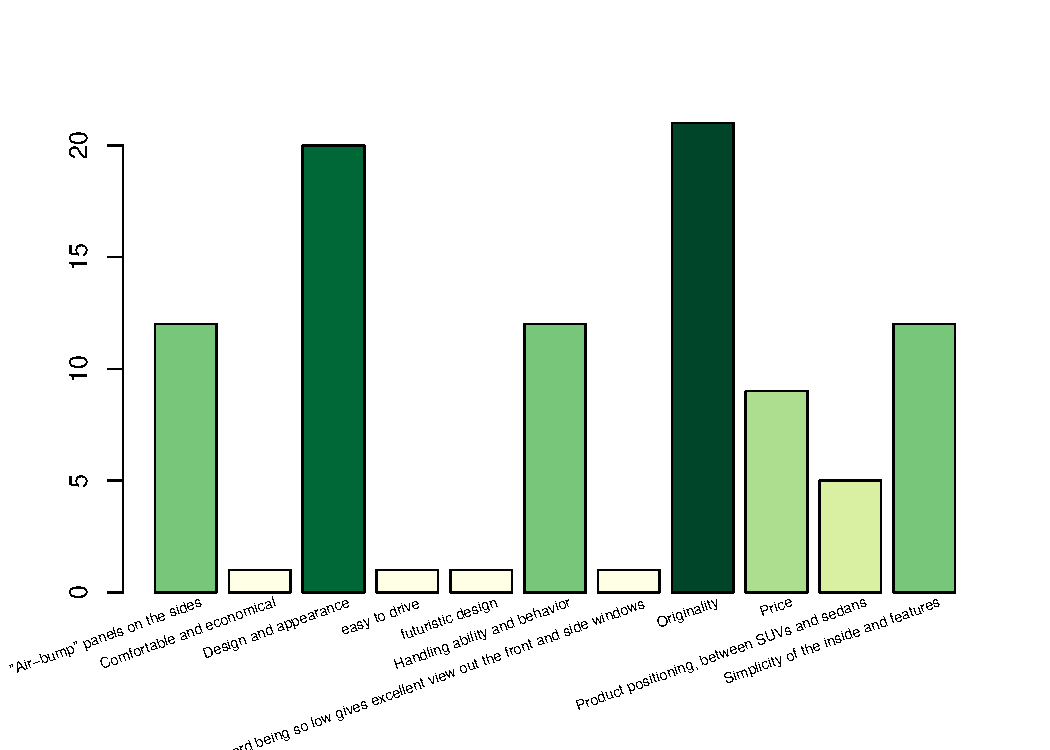
\includegraphics[width=\maxwidth]{figure/qualities_en-1} \caption[Qualités de la C4 Cactus selon les personnes ayant répondu au sondage anglais]{Qualités de la C4 Cactus selon les personnes ayant répondu au sondage anglais}\label{fig:qualities en}
\end{figure}


\end{knitrout}

\begin{knitrout}
\definecolor{shadecolor}{rgb}{0.969, 0.969, 0.969}\color{fgcolor}\begin{figure}[H]
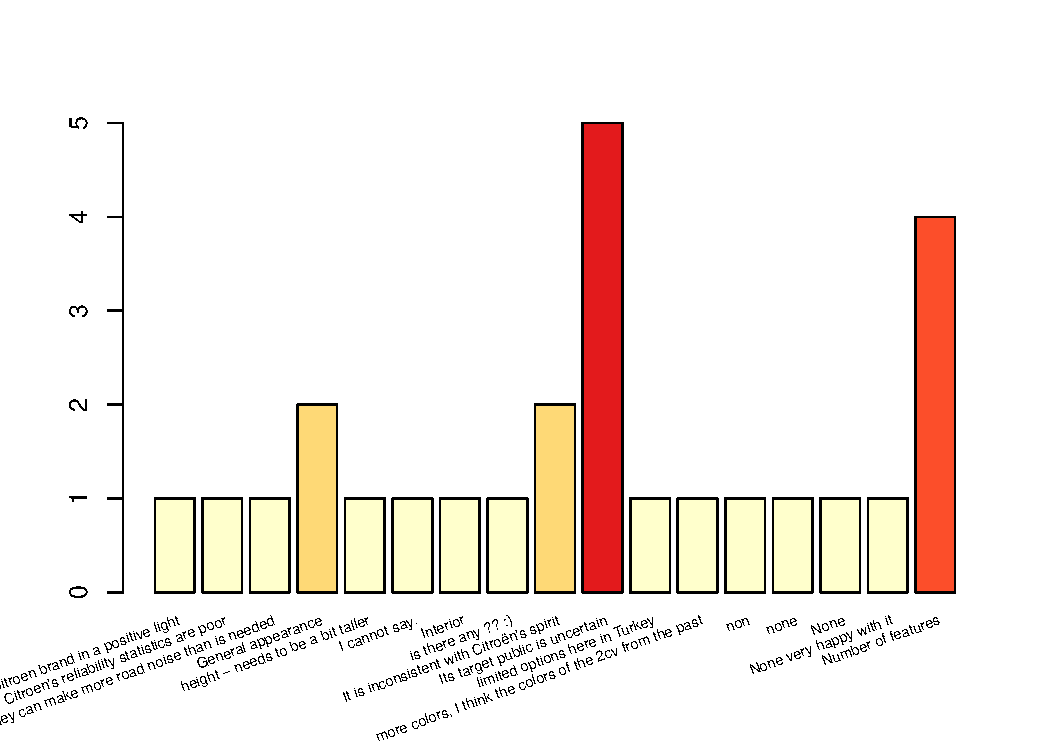
\includegraphics[width=\maxwidth]{figure/flaws_en-1} \caption[Défauts de la C4 Cactus selon les personnes ayant répondu au sondage anglais]{Défauts de la C4 Cactus selon les personnes ayant répondu au sondage anglais}\label{fig:flaws en}
\end{figure}


\end{knitrout}

\paragraph{} Pour les sondés à l'étranger, la
Citroën a plusieurs qualités qui sont son originalité, son design, son
comportement routier, la simplicité de son intérieur et de ses fonctionnalités
mais aussi ses airbumps. Cependant, 5 personnes trouvent que le public visé par
la marque est incertain, et 6 personnes trouvent que le nombre de
fonctionnalités est trop faible.

\begin{knitrout}
\definecolor{shadecolor}{rgb}{0.969, 0.969, 0.969}\color{fgcolor}\begin{figure}[H]
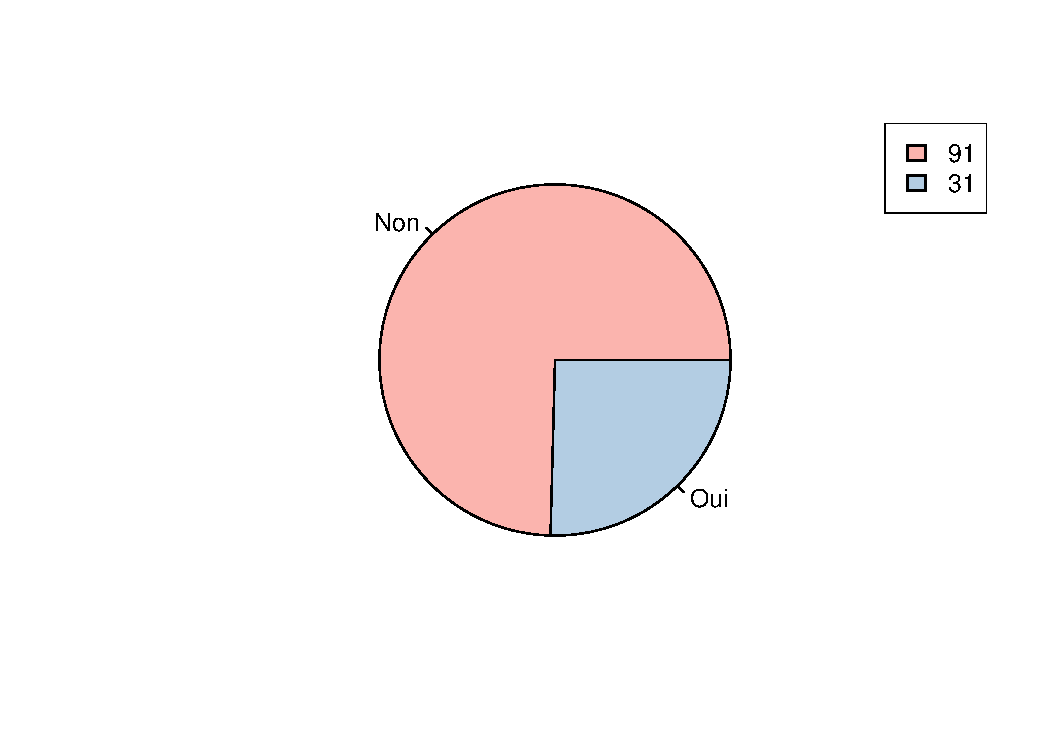
\includegraphics[width=\maxwidth]{figure/buy_fr-1} \caption[Proportion des personnes ayant répondu au sondage français et envisageant l'achat d'une C4 Cactus]{Proportion des personnes ayant répondu au sondage français et envisageant l'achat d'une C4 Cactus}\label{fig:buy fr}
\end{figure}


\end{knitrout}

%\begin{knitrout}
%\definecolor{shadecolor}{rgb}{0.969, 0.969, 0.969}\color{fgcolor}\begin{figure}[H]
%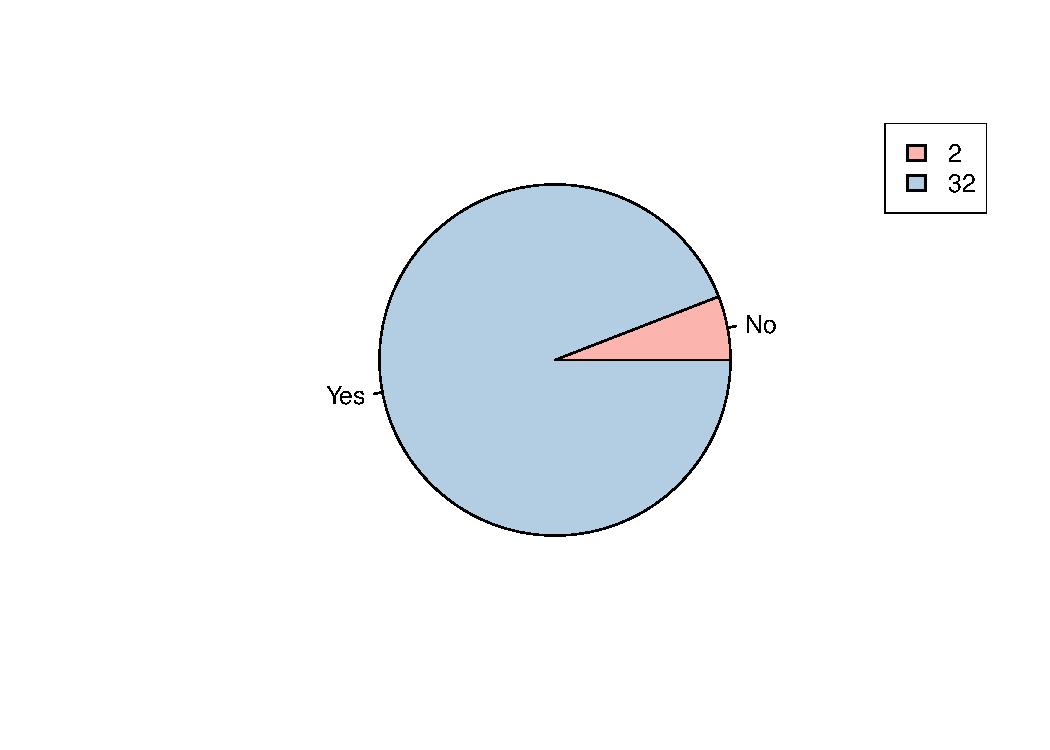
\includegraphics[width=\maxwidth]{figure/buy_en-1} \caption[Proportion des personnes ayant répondu au sondage anglais et envisageant l'achat d'une C4 Cactus]{Proportion des personnes ayant répondu au sondage anglais et envisageant l'achat d'une C4 Cactus}\label{fig:buy en}
%\end{figure}
%
%
%\end{knitrout}

\paragraph{} Pour conclure, un quart des Français
interrogés envisageraient d'acheter une C4 Cactus s'ils devaient acheter une automobile, alors
que 94\% des étrangers sondés feraient ce choix. Ce dernier chiffre est à confronter
au public ayant répondu à cette question, fidèle aux marques françaises et notamment à Citroën.

\break
\section{La marque DS}

\begin{knitrout}
\definecolor{shadecolor}{rgb}{0.969, 0.969, 0.969}\color{fgcolor}\begin{figure}[H]
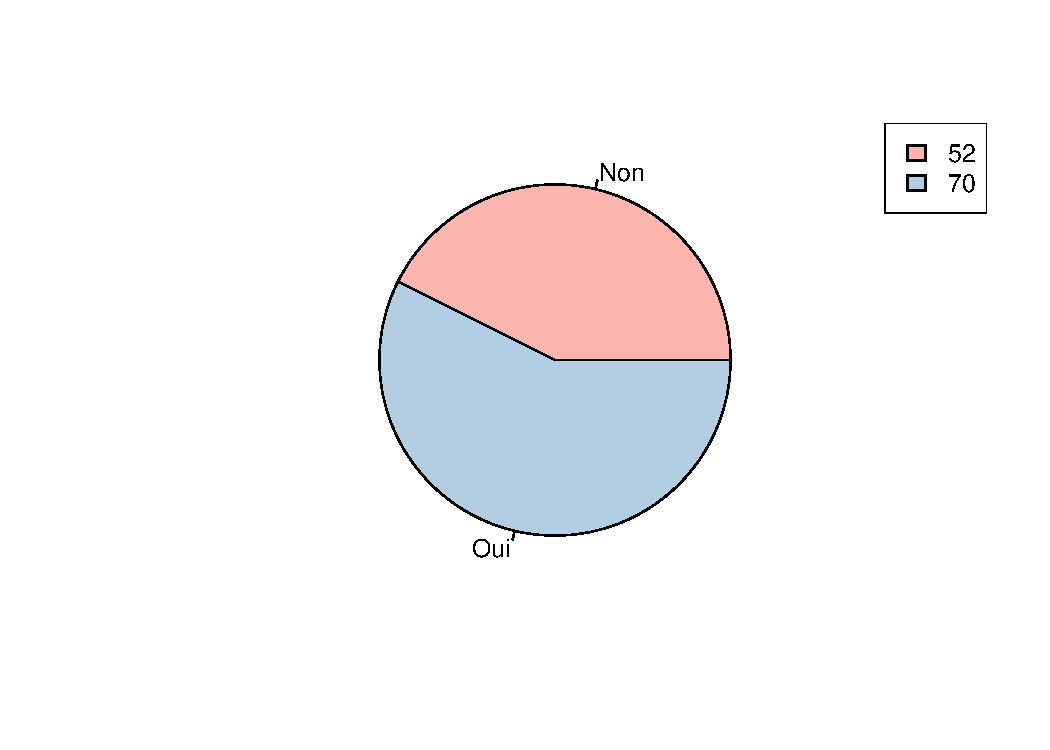
\includegraphics[width=\maxwidth]{figure/ds_know_fr-1} \caption[Proportion des personnes ayant répondu au sondage français et conscients de l'indépendance de DS]{Proportion des personnes ayant répondu au sondage français et conscients de l'indépendance de DS}\label{fig:ds know fr}
\end{figure}


\end{knitrout}

%\begin{knitrout}
%\definecolor{shadecolor}{rgb}{0.969, 0.969, 0.969}\color{fgcolor}\begin{figure}[H]
%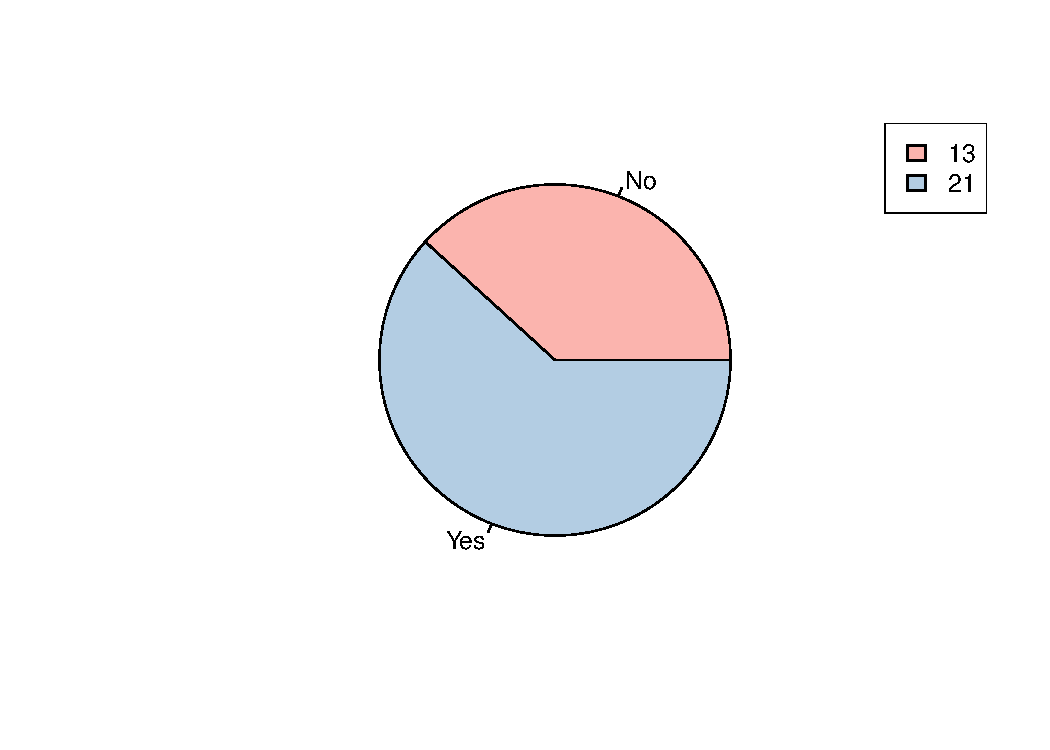
\includegraphics[width=\maxwidth]{figure/ds_know_en-1} \caption[Proportion des personnes ayant répondu au sondage anglais sachant que DS est une marque indépendante]{Proportion des personnes ayant répondu au sondage anglais et sachant que DS est une marque indépendante}\label{fig:ds know en}
%\end{figure}
%
%
%\end{knitrout}

\paragraph{} La part des Français conscients de l'indépendance de DS est
très similaire à celle des étrangers : 57 et 62\% respectivement. La divorce des
deux marques, voulu par PSA, n'est donc pas encore une évidence pour le public.

\begin{knitrout}
\definecolor{shadecolor}{rgb}{0.969, 0.969, 0.969}\color{fgcolor}\begin{figure}[H]
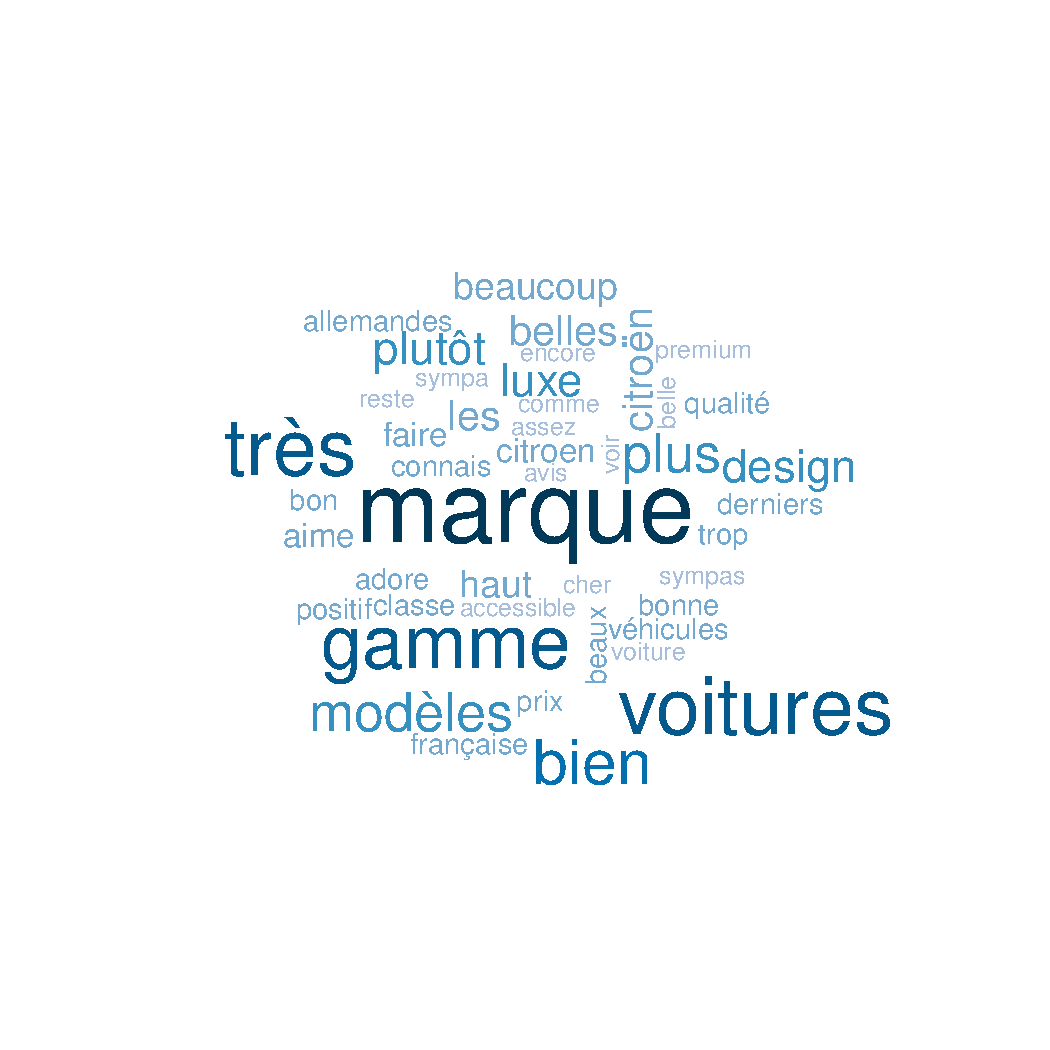
\includegraphics[width=\maxwidth]{figure/brand_fr-1} \caption[Nuage de mots de l'avis sur la marque DS des personnes ayant répondu au sondage français]{Nuage de mots de l'avis sur la marque DS des personnes ayant répondu au sondage français}\label{fig:brand fr}
\end{figure}


\end{knitrout}

%\begin{knitrout}
%\definecolor{shadecolor}{rgb}{0.969, 0.969, 0.969}\color{fgcolor}\begin{figure}[H]
%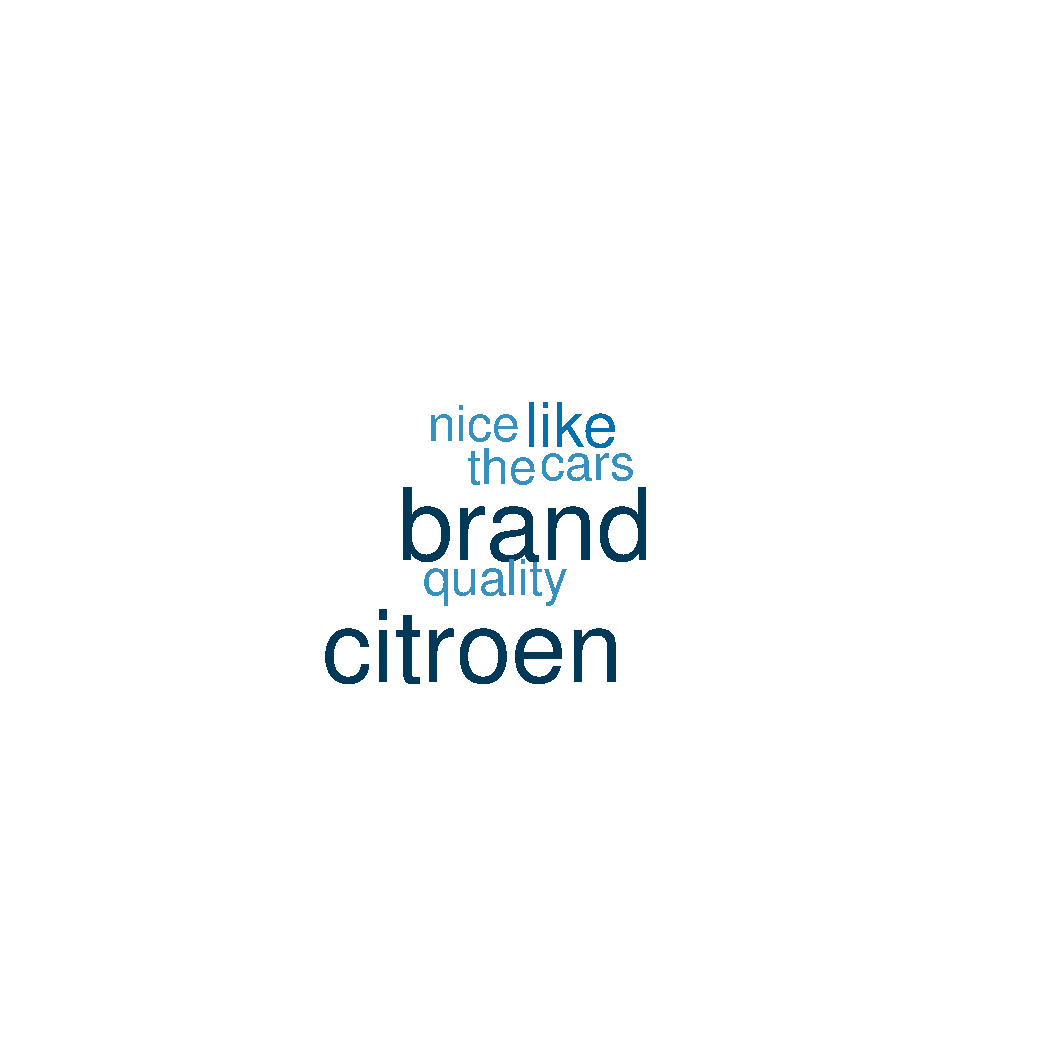
\includegraphics[width=\maxwidth]{figure/brand_en-1} \caption[Nuage de mots de l'avis sur la marque DS des personnes ayant répondu au sondage anglais]{Nuage de mots de l'avis sur la marque DS des personnes ayant répondu au sondage anglais}\label{fig:brand en}
%\end{figure}
%
%
%\end{knitrout}

\paragraph{} Concernant les avis sur la marque DS, le Français et les étrangers
sont d'accord sur un point : cette nouvelle marque incarne le luxe et un
design novateur et réussi, à un prix toutefois élevé.

\begin{knitrout}
\definecolor{shadecolor}{rgb}{0.969, 0.969, 0.969}\color{fgcolor}\begin{figure}[H]
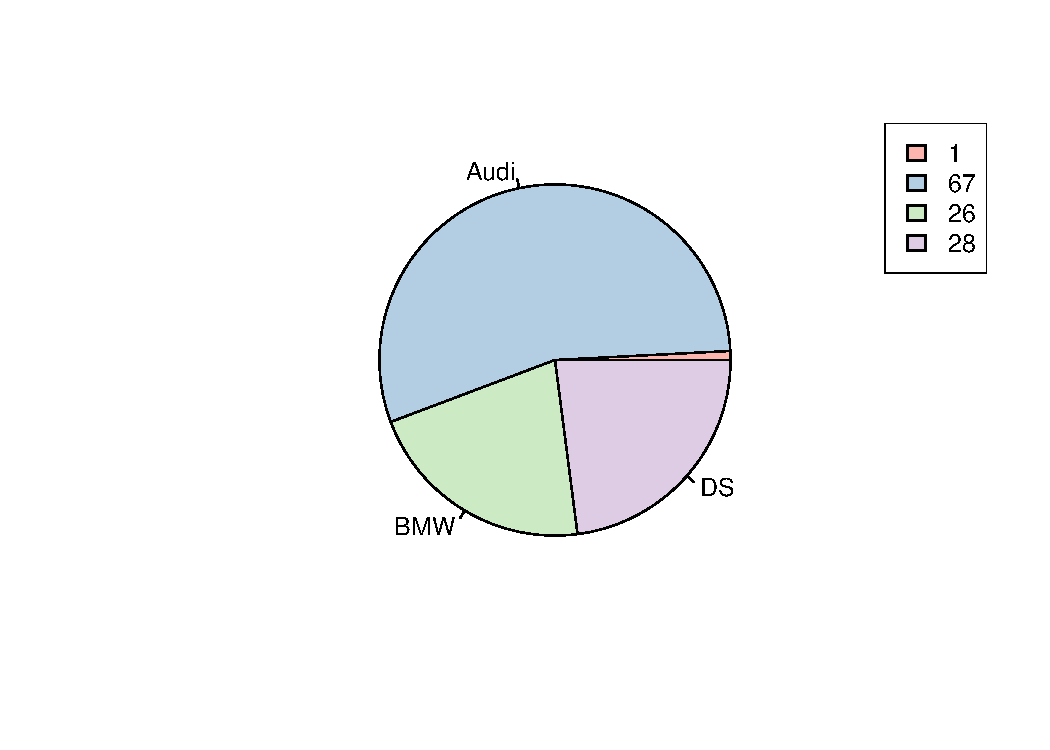
\includegraphics[width=\maxwidth]{figure/preference_fr-1} \caption[Réponses, chez les Français, à la question "Parmi ces trois marques, laquelle a votre préférence ?"]{Réponses, chez les Français, à la question "Parmi ces trois marques, laquelle a votre préférence ?"}\label{fig:preference fr}

\end{figure}


\end{knitrout}

\begin{knitrout}
\definecolor{shadecolor}{rgb}{0.969, 0.969, 0.969}\color{fgcolor}\begin{figure}[H]
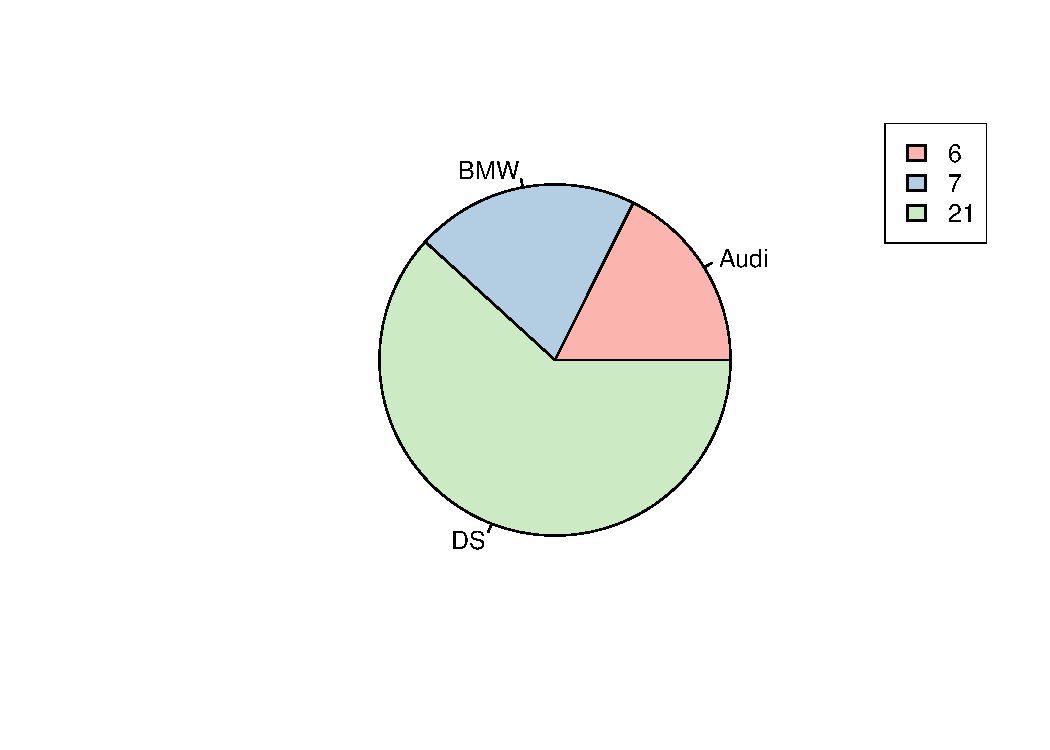
\includegraphics[width=\maxwidth]{figure/preference_en-1} \caption[Réponses, chez le public étranger, à la question "Parmi ces trois marques, laquelle a votre préférence ?"]{Réponses, chez le public étranger, à la question "Parmi ces trois marques, laquelle a votre préférence ?"}\label{fig:preference en}
\end{figure}


\end{knitrout}

\paragraph{} Cependant, les deux publics n'ont pas le même regard sur la concurrence
incarnée notamment par Audi et BMW, car si plus de la moitié des Français est
toujours attirée par Audi, les Britanniques sont eux en faveur de la marque française.

\break

\part{Conclusion}

\paragraph{} Un an après son lancement, la Citroën C4 Cactus ne se hisse qu'à la 22ème place des voitures les plus vendues en France depuis le début de l’année 2015. Ce succès mitigé peut s'expliquer en France par l'originalité du véhicule, dont le design s'éloigne des sentiers battus de Citroën. Si notre enquête a révélé que ce modèle proche des SUV rassemble de nombreux amateurs, il semble qu'il soit peu adapté au public français, moins amateur de SUV et souvent rebuté par l'aspect extérieur du véhicule et de ses \textit{airbumps}. Son prix, son confort et ses fonctionnalités en font un produit davantage destiné à des acheteurs à la recherche d'un véhicule utilitaire. Si l'objectif de Citroën était de proposer aux automobilistes français un nouveau type de véhicule quotidien, la Cactus paraît plus apte à conquérir le marché européen.


\paragraph{} La marque DS, quant à elle, s’est lancée sur le segment \textit{premium}, une gamme au dessus de la maison-mère Citroën ; un positionnement assumé par le prix et le design des véhicules. Elle veut incarner la voiture de luxe à la française et ainsi concurrencer les ténors européens Audi et BMW. Les résultats de nos sondages montrent que le jeune public français (20-30 ans) a plus d'affinités pour Audi que pour DS et BMW ; toutefois, il ne semble pas départager ces deux dernières. Ce constat permet de saluer une première réussite de DS, qui a su en quelques années s'approcher du niveau de popularité des marques \textit{premium} historiques. La marque s'offre ainsi les moyens de rivaliser avec Audi, BMW ou encore Lexus dans les années à venir, en profitant du renouvellement de leur public.


\paragraph{} Toutefois, alors que le public français plébiscite la prise d'indépendance de la marque, voyant Citroën sur une toute autre gamme, les amateurs de voitures françaises à l'étranger s'étonnent davantage de ce choix. Citroën a en effet conservé, notamment au Royaume-Uni, l'image de marque dont il jouissait entre 1960 et 1990 et dont la DS fait partie intégrante. Le groupe PSA Peugeot-Citroën doit donc relever un défi de communication : affirmer DS tout en redéfinissant Citroën, l'une comme égérie du luxe à la française, l'autre comme moteur d'innovation.

\printbibliography%

\end{document}

% vim: spell : spelllang=fr
